% chap3.tex
%

\mychapter{Structured and Unstructured Data for Factoid Question Answering}
\label{chapter:factoid}

\noindent

There are multiple ways to marry unstructured and structured data for joint question answering: convert structured data to unstructured format or vice versa, convert all data to certain intermediate representation or to leave them as is and link the data sources.
In my thesis I focus on two approaches: relation extraction for knowledge base completion, and semantic annotation of text for hybrid question answering.

\section{Relation Extraction for Knowledge Base Completion}
\label{sec:relation_extraction}

The information on the web is stored in multiple different forms, such as natural language statements, tables and infoboxes, images \etc.
In this work I focus on yet another source of information: question-answer pairs.
Community question answering archives contain hundreds of millions of question and corresponding answers.
Information expressed in these pairs might be hard to extract or not exist at all in other formats.

\subsection{Relation extraction from Question-Answer pairs}
\label{subsec:cqa_relextract}

CQA websites, such as Yahoo! Answers\footnote{http://answers.yahoo.com/}, Answers.com\footnote{http://www.answers.com}, Quora\footnote{http://quora.com} \etc, has gained a lot of popularity in the recent years, and their archives store hundreds of millions of user questions along with answers provided by the community.
Many users' information needs are not unique and arise again and again, which makes it possible to reuse the information to answers new questions \cite{Shtok:2012:LPA:2187836.2187939}.
This idea makes CQA data attractive for knowledge base population.
Although some of the facts mentioned in QnA pairs can also be found in some other text documents, another part might be unique (\eg in Clueweb\footnote{http://www.lemurproject.org/clueweb12/} about 10\% of entity pairs with existing Freebase relations mentioned in Yahoo! Answers documents cannot be found in other documents \cite{savenkov2015relation}).
Existing relation extraction techniques face some challenges when applied to CQA data, \ie they typically consider sentences independently and ignore the discourse of a QnA pair text.
However, frequently, it is impossible to understand the answer without knowing the question.
For example, sometimes users simply give the answer to the question without stating it in a narrative sentence (\eg ``\emph{What does "xoxo" stand for? Hugs and kisses.}``), or the provided answer might contain ellipsis, \ie some important information is omitted (\eg ``\emph{What's the capital city of Bolivia? Sucre is the legal capital, though the government sits in La Paz}``).

In this thesis we propose a novel model for relation extraction from CQA data, that uses discourse of a QnA pair to extract facts between entities mentioned in question and entities mentioned in answer sentences.
The conducted experiments confirm that many of such facts cannot be extracted by existing sentence-based techniques and thus it is beneficial to combine their outputs with the output of our model. 

Let us define the problem more formally.
We target the problem of relation extraction from QnA data, which is a collection of $(q, a)$ pairs, where $q$ is a question text (can contain multiple sentences) and $a$ is the corresponding answer text (can also contain multiple sentences).
By relation instance $r$ we mean an ordered binary relation between $subject$ and $object$ entities, which is commonly represented as $[subject, predicate, object]$ triple.
For example, the fact that Brad Pitt married Angelina Jolie can be represented as [Brad Pitt, married\_to, Angelina Jolie].
In this work we use Freebase, an open schema-based KB, where all entities and predicates come from the fixed alphabets $E$ and $P$ correspondingly.
% The relation extraction problem can be formulated as a multiple instance multi-label classification problem \cite{Surdeanu:2012:MML:2390948.2391003}.
Let $e_1$ and $e_2$ be entities that are mentioned together in a text (\eg in a sentence, or $e_1$ in a question and $e_2$ in the corresponding answer), we will call such an entity pair with the corresponding context a mention.
The same pair of entities can be mentioned multiple times within the corpus, and for all mentions $i=1,...,n$ the goal is to predict the expressed predicate ($z_i \in P$) or to say that none applies ($z_i = \emptyset$).
Individual mention predictions $z_1, ..., z_n$ are combined to infer a set of relations $\mathbf{y}=\{y_i \in P\}$ between the entities $e_1$ and $e_2$.

\begin{figure}[h]
\centering
\begin{tikzpicture}
\tikzstyle{main}=[circle, minimum size = 8mm, thick, draw =black!80, node distance = 14mm]
\tikzstyle{mainnob}=[circle, minimum size = 8mm, thick, draw =white!100, node distance = 14mm]
\tikzstyle{connect}=[-latex, thick]
\tikzstyle{box}=[rectangle, draw=black!100]
\node[main, fill = white!100] (y) [label=center:$y$] { };
\node[rectangle, inner sep=-1mm, fit=(y),label=below right:$P$] {};
\node[rectangle, inner sep=4mm, fit=(y),draw=black!100] {};
\node[main, fill = white!100] (z) [below=of y,label=center:$z$] { };
%\node[rectangle, inner sep=-1mm, fit=(z),label=below right:$P$] {};
%\node[rectangle, inner sep=4mm, fit=(z),draw=black!100] {};
\node[main, fill = black!10] (x) [below=of z,label=center:$\mathbf{x}$] { }; 
\node[main, fill = black!10] (t) [right=of z,label=center:$\mathbf{x_t}$] { };
\node[mainnob, fill = white!100] (wt) [right=of y,label=center:$\mathbf{w_t}$] { };
\node[mainnob, fill = white!100] (wx) [left=of y,label=center:$\mathbf{w_x}$] { };
\node[rectangle, inner sep=-1mm, fit=(z)(x)(t),label=below right:$|Q|$, yshift=-1mm] {};
\node[rectangle, inner sep=6.5mm, fit=(z)(x)(t),draw=black!100] {};

\node[rectangle, inner sep=-1mm, fit=(z)(x),label=below right:$M$,yshift=-12mm] {};
\node[rectangle, inner sep=5.0mm, fit=(z)(x),draw=black!100] {};

\node[rectangle, inner sep=-1mm, fit=(x)(z)(y),label=below right:$N$,yshift=-30mm,xshift=4.5mm] {};
\node[rectangle, inner sep=9mm, fit=(x)(z)(y),draw=black!100, yshift=-3mm] {};

\path (wx) edge [connect] (z)
(x) edge [connect] (z)
(z) edge [connect] (y)
(wt) edge [connect] (z)
(t) edge [connect] (z);
\end{tikzpicture}
\vspace{-15mm}
\caption{QnA-based relation extraction model plate diagram.
$N$ - number of different entity pairs, $M$ - number of mentions of an entity pair, $|Q|$ - number of questions where an entity pair is mentioned, $\mathbf{x}$ and $\mathbf{x_t}$ - mention-based and question-based features, $\mathbf{w}$ and $\mathbf{w_t}$ - corresponding feature weights, latent variables $z$ - relation expressed in an entity pair mention, latent variables $y$ - relations between entity pair}
\label{fig:qna_relextract:graphmodel}
\end{figure}

Our models for relation extraction from QnA data incorporates the topic of the question and can be represented as a graphical model (Figure \ref{fig:qna_relextract:graphmodel}).
Each mention of a pair of entities is represented with a set of mention-based features $x$ and question-based features $x_t$.
A multinomial latent variable $z$ represents a relation (or none) expressed in the mention and depends on the features and a set of weights $w_x$ for mention-based and $w_t$ for question-based features:
$$\hat{z}=\argmax{z \in P \cup \emptyset} p(z|x, x_t, w_x, w_t)$$.
To estimate this variable we use L2-regularized multinomial logistic regression model, trained using the distant supervision approach for relation extraction \cite{MintzBSJ09}, in which mentions of entity pairs related in Freebase are treated as positive instances for the corresponding predicates, and negative examples are sampled from mentions of entity pairs which are not related by any of the predicates of interest.
Finally, to predict a set of possible relations $\mathbf{y}$ between the pair of entities we take logical OR of individual mention variables $\mathbf{z}$, \ie $y_p = \lor_{i=1}^M [z_i = p, p \in P]$, where M is the number of mentions of this pair of entities.

\subsubsection{Sentence-based baseline model}

Existing sentence-based relation extraction models can be applied to individual sentences of a QnA pair and will work well for complete statements, \eg ``Who did Brad Pitt marry? Brad Pitt and Angelina Jolie married at secret ceremony''.
In sentence-based scenario, when the set of question-based features is empty, the above model corresponds to the Mintz++ baseline described in \cite{Surdeanu:2012:MML:2390948.2391003}, which was shown to be superior to the original model of \cite{MintzBSJ09}, is easier to train than some other state of the art distant supervision models and produces comparable results.

\subsubsection{Sentence-based model with question features}

\begin{table*}[tbh]
\centering
\caption{Examples of features used for relation extraction for ``\emph{When was Mariah Carey born? Mariah Carey was born 27 March 1970}''}
\vspace{-2mm}
\label{table:qna_relextract:features}
\begin{tabular}{|p{8cm}|p{8cm}|}
\hline
\multicolumn{2}{|c|}{Sentence-based model}\\
\hline
Dependency path between entities & [PERSON]$\rightarrow$nsubjpass(born)tmod$\leftarrow$[DATE]\\
Surface pattern & [PERSON] be/VBD born/VBN [DATE]\\
\hline
\hline
\multicolumn{2}{|c|}{Question features for sentence-based model}\\
\hline
Question template & when [PERSON] born\\
Dependecy path from a verb to the question word & (when)$\rightarrow$advmod(born)\\
Question word + dependency tree root & when+born\\
\hline
\hline
\multicolumn{2}{|c|}{QnA-based model}\\
\hline
Question template + answer entity type & Q: when [PERSON] born A:[DATE]\\
Dependency path from question word to entity & Q:(when)$\rightarrow$advmod(born)nsubj$\leftarrow$[PERSON]\\
and answer entity to the answer tree root & A: (born)tmod$\leftarrow$[DATE]\\
Question word, dependency root and answer pattern & Q: when+born A:born [DATE]\\
\hline
\end{tabular}
\end{table*}

In many cases an answer statement is hard to interpret correctly without knowing the corresponding question.
To give the baseline model some knowledge about the question, we include question features (Table \ref{table:qna_relextract:features}), which are based on dependency tree and surface patterns of a question sentence. 
This information can help the model to account for the question topic and improve predictions in some ambiguous situations.

\subsubsection{QnA-based model}
The QnA model for relation extraction is inspired by the observation, that often an answer sentence do not mention one of the entities at all, \eg, ``\textit{When was Isaac Newton born? December 25, 1642 Woolsthorpe, England}''.
To tackle this situation we make the following assumption about the discourse of a QnA pair: an entity mentioned in a question is related to entities in the corresponding answer and the context of both mentions can be used to infer the relation predicate.
Our QnA-based relation extraction model takes an entity from a question sentence and entity from the answer as a candidate relation mention, represents it with a set features (Table \ref{table:qna_relextract:features}) and predicts a possible relation between them similar to sentence-based models.
The features are conjunctions of various dependency tree and surface patterns of question and answer sentences, designed to capture their topics and relation.

\subsubsection{Experiments}

For experiments we used 2 publicly available CQA datasets: Yahoo! Answers WebScope dataset\footnote{http://webscope.sandbox.yahoo.com/catalog.php?datatype=l} and a crawl of WikiAnswers\footnote{http://wiki.answers.com/} collected by \cite{Fader:2014:OQA:2623330.2623677}.
The Yahoo! Answers dataset contains 4,483,032 questions (3,894,644 in English) with the corresponding answers collected on 10/25/2007.
The crawl of WikiAnswers has 30,370,994 question clusters, tagged by WikiAnswers users as paraphrases, and only 3,386,256 them have answers.
From these clusters we used all possible pairs of questions and corresponding answers (19,629,443 pairs in total).

\begin{table*}[ht]
\centering
\caption{Yahoo! Answers and WikiAnswers datasets statistics}
\vspace{-2mm}
\label{table:qna_relextract:cqastats}
\begin{tabular}{|p{12.5cm}||p{1.2cm}|p{1.2cm}|} \hline
& Y!A & WA\\
\hline
Number of QnA pairs & 3.8M & 19.6M \\
Average question length (in chars) & 56.67 & 47.03 \\
Average answer length (in chars) & 335.82 & 24.24 \\
% Number of resolved entities per QnA pair & 3.57 & 3.23 \\
Percent of QnA pairs with answers that do not have any verbs & 8.8\% & 18.9\% \\
Percent of QnA pairs with at least one pair of entities related in Freebase & 11.7\% & 27.5\% \\
Percent of relations between entity pairs in question sentences only & 1.6 \% & 3.1\% \\
Percent of relations between entity pairs in question and answer sentences only & 28.1\% & 46.4\% \\
Percent of relations between entity pairs in answer sentences only & 38.6\%& 12.0\%\\
\hline
\end{tabular}
\end{table*}

For each QnA pair we applied tokenization, sentence detection, named entity tagger, parsing and coreference resolution from Stanford CoreNLP \cite{manning-EtAl:2014:P14-5}.
Our cascade entity linking approach is similar to \cite{chang2011stanford} and considered all noun phrase and named entity mentions as candidates.
First all named entity mentions are looked up in Freebase names and aliases dictionary.
The next two stages attempt to match mention text with dictionary of English Wikipedia concepts \cite{spitkovsky2012cross} and its normalized version.
Finally for named entity mentions we try spelling correction using Freebase entity names dictionary.
We didn't disambiguate entities and instead took top-5 ids for each coreference cluster (using the $p(entity|phrase)$ score from the dictionary or number of existing Freebase triples).
All pairs of entities (or entity and date) in a QnA pair that are directly related\footnote{We also consider some paths that come through a mediator node, \eg  /people/person/spouse\_s./people/marriage/spouse} in Freebase were annotated with the corresponding relations.

Table \ref{table:qna_relextract:cqastats} gives some statistics on the datasets used in this work.
The analysis of answers that do not have any verbs show that $\sim$8.8\% of all QnA pairs do not state the predicate in the answer text.
The percentage is higher for WikiAnswers, which has shorter answers on average.
Unfortunately, for many QnA pairs we were unable to find relations between the mentioned entities (for many of them no or few entities were resolved to Freebase).
Among those QnA pairs, where some relation was annotated, we looked at the location of related entities.
In Yahoo! Answers dataset 38.6\% (12.0\% for WikiAnswers) of related entities are mentioned in answer sentences and can potentially be extracted by sentence-based model, and 28.1\% (46.4\% for WikiAnswers) between entities mentioned in question and answer sentences, which are not available to the baseline model and our goal is to extract some of them.

For our experiments we use a subset of 29 Freebase predicates that have enough unique instances annotated in our corpus, \eg date of birth, profession, nationality, education institution, date of death, disease symptoms and treatments, book author, artist album, \etc
We train and test the models on each dataset separately.
Each corpus is randomly split for training (75\%) and testing (25\%).
Knowledge base facts are also split into training and testing sets (50\% each).
QnA and sentence-based models predict labels for each entity pair mention, and we aggregate mention predictions by taking the maximum score for each predicate.
We do the same aggregation to produce a combination of QnA- and sentence-based models, \ie, all extractions produced by the models are combined and if there are multiple extractions of the same fact we take the maximum score as the final confidence.
The precision and recall of extractions are evaluated on a test set of Freebase triples, \ie an extracted triple is considered correct if it belongs to the test set of Freebase triples, which are not used for training (triples used for training are simply ignored).
Note, that this only provides a lower bound on the model performance as some of the predicted facts can be correct and simply missing in Freebase.

Figure \ref{fig:qna_relextract:pr_curve} shows Precision-Recall curves for QnA-based and sentence-based baseline models and some numeric results are given in Table \ref{table:qna_relextract:results}.
As 100\% recall we took all pairs of entities that can be extracted by either model.
It is important to note, that since some entity pairs occur exclusively inside the answer sentences and some in pairs of question and answer sentences, none of the individual models is capable of achieving 100\% recall, and maximum possible recalls for QnA- and sentence-based models are different.

\begin{figure}[h!]
\centering
\vspace{-2mm}
\begin{subfigure}[h]{0.45\textwidth}
	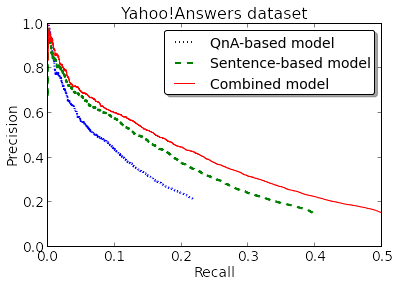
\includegraphics[width=0.99\textwidth]{img/qa_vs_sent_ya}
	\vspace{-1mm}
    \label{figure:pr:ya}
\end{subfigure}
\begin{subfigure}[h]{0.45\textwidth}
	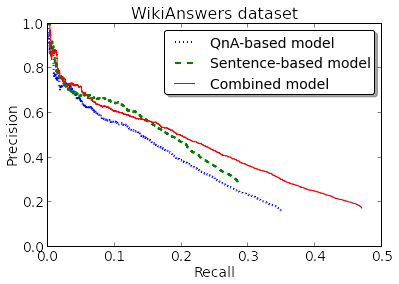
\includegraphics[width=0.99\textwidth]{img/qa_vs_sent_wa}
	\vspace{-1mm}
    \label{figure:pr:wa}
\end{subfigure}
\begin{subfigure}[h]{0.45\textwidth}
	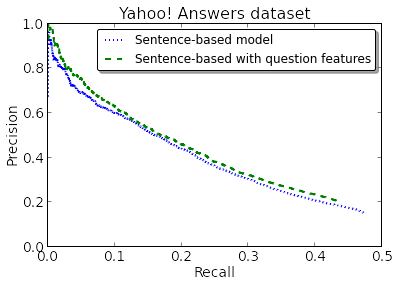
\includegraphics[width=0.99\textwidth]{img/noqf_vs_qf}
	\vspace{-1mm}
	\label{figure:pr:noqf_vs_qf}
\end{subfigure}
\vspace{-1mm}
\caption{Precision-Recall curves for QnA-based vs sentence-based models and sentence-based model with and without question features}
\label{fig:qna_relextract:pr_curve}
\end{figure}

\begin{table*}[tbh]
\centering
\caption{Extraction results for QnA- and sentence-based models on both datasets}
\vspace{-2mm}
\label{table:qna_relextract:results}
\begin{tabular}{|p{6.6cm}||p{0.9cm}|p{1.4cm}|p{1.6cm}||p{0.9cm}|p{1.4cm}|p{1.6cm}|}
\hline
& \multicolumn{3}{|c||}{Yahoo! Answers} & \multicolumn{3}{|c|}{WikiAnswers}\\
\cline{2-7}
& QnA & Sentence & Combined & QnA & Sentence & Combined\\
\hline
F-1 score & 0.219 & 0.276 & 0.310 & 0.277 & 0.297 & 0.332\\
Number of correct extractions & 3229 & 5900 & 7428 & 2804 & 2288 & 3779 \\
Correct triples not extracted by other model & 20.5\% & 56.5\% & - & 39.4\% & 25.8\% & - \\
\hline
\end{tabular}
\end{table*}

Results demonstrate that from 20.5\% to 39.4\% of correct triples extracted by the QnA-based model are not extracted by the baseline model, and the combination of both models is able to achieve higher precision and recall.
Unfortunately, comparison of sentence-based model with and without question-based features (Figure \ref{fig:qna_relextract:pr_curve}) didn't show a significant difference.

\subsubsection{Analysis}

To get an idea of typical problems of QnA-based model we sampled and manually judged extracted high confidence examples that are not present in Freebase (and thus are considered incorrect for precision-recall analysis).

The major reason (40\%) of false positive extractions is errors in entity linking.
For example: ``\emph{Who is Tim O'Brien? He was born in Austin on October 1, 1946}''.
The model was able to correctly extract [Tim O'Brien, date\_of\_birth, October 1, 1946], however Tim O'Brien was linked to a wrong person.
In a number of cases (16\%) our discourse model turns out to be too simple and fails for answers, that mention numerous additional information, \eg ``\emph{How old is Madonna really? ...Cher was born on 20 May 1946 which makes her older that Madonna...}''.
A possible solution would be to either restrict QnA-based model to cases when no additional information is present or design a better discourse model with deeper analysis of the answer sentence and its predicates and arguments.
Some mistakes are due to distant supervision errors, for example for the music.composition.composer predicate our model extracts singers as well as composers (which are in many cases the same).

Of course, there are a number of cases, when our extractions are indeed correct, but are either missing (33\%) or contradicting with Freebase (8\%).
An example of an extracted fact, that is missing in Freebase is ``\emph{Who is Wole Soyinka? He studied at the University College, Ibadan(1952-1954) and the University of Leeds (1954-1957)}'', and [Wole Soyinka, institution, University of Leeds] is currently not present in Freebase.
Contradictions with Freebase occur because of different precision levels (``pianist'' vs ``jazz pianist'', city vs county, \etc), different calendars used for dates or ``incorrect'' information provided by the user.
An example, when existing and extracted relation instance are different in precision is:``\emph{Who is Edward Van Vleck? Edward Van Vleck was a mathematician born in Middletown, Connecticut}'' we extract [Edward Van Vleck, place\_of\_birth, Middletown], however the Freebase currently has USA as his place of birth.

The problem of ``incorrect'' information provided in the answer is very interesting and worth special attention.
It has been studied in CQA research, \eg \cite{shah2010evaluating}, and an example of such QnA pair is: ``\emph{Who is Chandrababu Naidu? Nara Chandra Babu Naidu (born April 20, 1951)}''.
Other authoritative resources on the Web give April 20, 1950 as Chandrababu Naidu's date of birth.
This raises a question of trust to the provided answer and expertise of the answerer.
Many questions on CQA websites belong to the medical domain, \eg people asking advices on different health related topics.
How much we can trust the answers provided to extract them into the knowledge base?
We leave this question to the future work.

Finally, we have seen that only a small fraction of available QnA pairs were annotated with existing Freebase relations, which shows a possible limitation of Freebase schema.
A promising direction for future work is automatic extraction of new predicates, which users are interested in and which can be useful to answer more future questions.

\subsubsection{Conclusion}

In this section we described a model for relation extraction from QnA data, which is capable of predicting relations between entities mentioned in question and answer sentences.
We conducted experiments on 2 publicly available CQA datasets and showed that our model can extract triples not available to existing sentence-based techniques and can be effectively combined with them for better coverage of a knowledge base population system.


% BELOW IS MY ANOTHER IDEA, BUT IT'S VAGUE AND DOESN'T HAVE ANY CONCRETE PLAN
% \subsection{Question-guided relation extraction}
%\label{subsec:question_based_relextract}
%The idea is that we can aggregate related questions and relation extraction patterns.
%When a person asks a question, we retrieve passages and sentences to extract the answer from.
%Imaging a question is asking a certain property of an entity.
%If we can retrieve a sentence, that mentions this entity along with a candidate answer, we can build a pattern for relation extraction.
%This pattern will be connected to the question ``template''.
%Likewise, if we already have relation extraction patterns we can boost those that are retrieve in response to the question and save this connection.

%Hypothesis:
%\begin{enumerate}
%\item Patterns retrieved in response to the question are better in quality, we can boost them. We can try to verify this on some relation extraction dataset and questions from some query log. We can also try to use some KBQA dataset.
%\item Patterns mined for questions should help question answering. This is essentially weak supervision for training knowledge base question answering using text based question answering.
%\end{enumerate}

%Problems:
%\begin{itemize}
%\item How to extract new predicates? If we have a question, and a sentence is mentioning a pair of non-related entities, how can we make a new one?
%\item How to deal with more complex questions, that are not simple relations
%\end{itemize}

%Useful dataset: MSN query log, SimpleQuestions from Facebook, WebQuestions, NYT relation extraction dataset.

%This approach can also be applied to open IE.
%There are sentence selection methods for question answering.
%We can extract noun phrases (NP mentioned in question and supposedly answer NP), and then aggregate all sentences, that mention the same NPs together.
%Hypothesis is, that we can extract patterns, that will answer the same question for other entities.

\section{Semantic Text Annotations for Hybrid Question Answering}
\label{sec:text+kb}

Converting unstructured information into structured form by extracting knowledge from text suffers from certain quality losses.
Existing relation extraction tools aren't perfect, in particular due to recall losses a lot of information is left behind.
Moreover, extractions contain certain level of incorrect information due to precision losses.
These errors cap the upper bound on the question answering system performance.

Here I propose to utilize the synergy of structured and unstructured data, and exploit the advantages of each of them to overcome the limitations of the other.
More particularly, I propose to annotate and index mentions of knowledge base entities in text documents, which essentially induce a special kind of edges to the knowledge base, and allows one to traverse these edges in both directions.
These links open up many opportunities for QA reasoning, \eg retrieving all the information about the entity by going from a mention to a KB entity, finding relations between entities by retrieving text passages that mention both of them, extracting candidate evidence by retrieving passages that mention question and answer entities along with some question terms, and so on.
First, in Section \ref{subsec:text2kb} we describe how external text data can help to improve the performance of knowledge base question answering, and in Section \ref{subsec:text+kb} I propose a novel hybrid question answering architecture.

\subsection{Text2KB: Knowledge Base Question Answering using External Text Data}
\label{subsec:text2kb}




\subsection{Hybrid Question Answering over Knowledge Bases and Semantically Annotated Text Collections}
\label{subsec:text+kb}

\begin{figure*}
\centering
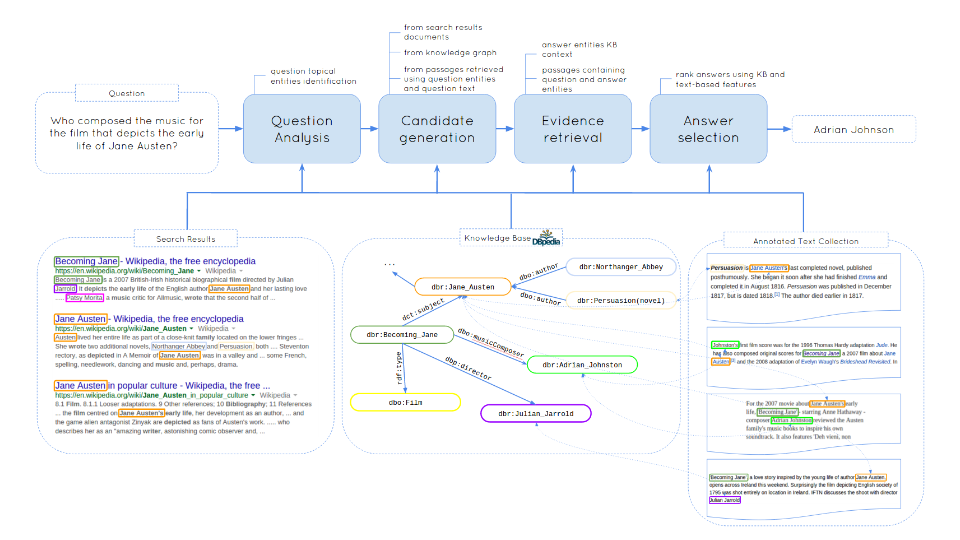
\includegraphics[width=\textwidth]{img/text_and_kb}
\caption{Architecture of a hybrid factoid question answering system, that uses a combination of structured knowledge base and unstructured text data}
\label{fig:text_kb}
\end{figure*}

The architecture of the hybrid QA model I propose is presented on Figure \ref{fig:text_kb}.
Here are the main stages of the question answering process:
\begin{itemize}
\setlength\itemsep{0em}
\item \textbf{Pre-processing}: identify mentions of KB entities in text document collection and index the documents text and mentions in separate fields
\item \textbf{Topical entity identification}: search the text collection using question (or reformulated question \cite{AgichteinLG01}) as a query and use an approach similar to \cite{cornolti2014smaph} to detect question topical entities
\item \textbf{Candidate generation from text}: extract candidate answer (or intermediate answer) entities with evidence from the retrieved text documents using existing techniques, e.g. \cite{tsai2015web}.
\item \textbf{Candidate generation from KB}: explore the KB neighborhood of question topical entities and entities extracted from text documents on the previous step
\item \textbf{Candidate generation from KB \& Text}: use entity and text index to find entities mentioned near question topical entity and question terms in the document collection
\item \textbf{KB evidence extraction}: match neighborhood of answer entities (entity type and other entities) against the question to get additional evidence
\item \textbf{Text evidence extraction}: estimate the similarity between the collection text fragments mentioning question and answer entities and the question text
\item \textbf{Rank candidate}: rank candidate answers using evidence extracted from the KB as well as from text
\end{itemize}

Let's consider an example question ``\textit{Who composed the music for the film that depicted the early life of Jane Austen?}'' from the QALD dataset\footnote{http://greententacle.techfak.uni-bielefeld.de/~cunger/qald/} (Figure \ref{fig:text_kb}).
Even though it's quite easy to identify the ``\texttt{Jane Austen}'' entity in the question, the knowledge base (dbPedia in this example) cannot help us to determine which movie is being referred to.
However, there are a lot of documents on the web, that do mention the ``\texttt{Becoming Jane}'' movie and say what is it about.
Unfortunately, extracting the name of the composer from these documents is quite challenging, but this task can be easily accomplished by checking the value of the \texttt{musicComposer} property in the knowledge base.
At the end, for each candidate answer entity, we have all the KB information and passages that mention this entity as evidence to help with the correct answer selection.

\subsubsection{Evaluation}
\label{sec:factoid_evaluation}


I THINK HERE WE CAN INCLUDE OUR RESULTS ON TEXT2KB.

Most of the recent work on knowledge base question answering and semantic parsing have been evaluated on the WebQuestions dataset \cite{BerantCFL13:sempre}, which contains a collection of question text and correct answer entities.
The questions were collected using Google Suggest API and answers crowdsourced using Amazon Mechanical Turk\footnote{http://mturk.com/}
The proposed approach will be compared against the previous results\footnote{http://goo.gl/sePBja} on this dataset.
Again, web can be used as a text collection which can be queried using Bing Search API.
Relation extraction patterns can be mined using distant supervision from ClueWeb collection using publicly available dataset of Freebase annotations \cite{gabrilovich2013facc1}.

\textbf{New factoid question answering dataset}.
However, WebQuestions dataset has certain limitations, e.g. questions mined using Google Suggest API have very similar structure and lexicon, and to find the answer to the mined questions users were asked to use the question entity Freebase profile page,  which only include entities connected directly with a predicate or through a mediator node.
Therefore most of the state-of-the-art results on the dataset use a small number of predefined logical form patterns.
On the other hand CQA websites have a fraction of factoid questions with provided text answers.
Here I propose to use to construct a new dataset for question answering over Freebase by selecting a subset of QnA pairs with at least one entity in question and answer and some reasonable filtering heuristics and manual validation using crowdsourcing (e.g. through Amazon Mechanical Turk).
Existing systems need to be retrained and tested on the new dataset to compare against the proposed model.

...........

TREC QA datasets served as a benchmark for various question answering systems.
Therefore, to evaluate the proposed approach for question answering over text enriched with the structured data I propose to test it on dataset derived from TREC QA and compare against existing strong baselines, including the most related approaches \cite{Fader:2014:OQA:2623330.2623677,Sun:2015:ODQ:2736277.2741651}.
The proposed system can use the web as the corpus and query it using Bing Search API\footnote{https://datamarket.azure.com/dataset/bing/searchweb}.
Freebase and Reverb extractions \cite{FaderSE11} are examples of schema-based and open knowledge bases that can be used for the experiments.
The metrics used for evaluation typically include accuracy and mean reciprocal rank (MRR).

For non-factoid question answering this year TREC pioneered a new question answering track - TREC LiveQA\footnote{http://trec-liveqa.org/}, which targets questions asked by real users of Yahoo! Answers website.
This year the deadline for system submission was on August 31 and my system trained on CQA QnA pairs participated in the challenge.
The results will be available on the TREC Conference in November 2015.
Organizers plan to continue with another TREC LiveQA task next year and this is going to be a good estimation of the effectiveness of the proposed techniques on hard real user questions.


\section{Summary}
In this section we considered two different ways of combining unstructured and structured data to improve factoid question answering.
Relation extraction from question-answer pairs aims at filling some gaps in KB fact coverage, whereas semantic annotations of text documents provides a way to incorporate information available in unstructured text documents for reasoning along with KB data to improve the performance of factoid question answering.

Factoid questions represent just a part of user information needs. Many problems require more elaborate response, such as a sentence, list of instructions or in general a passage of text.
Such questions are usually referred to as non-factoid questions and they will be the focus of the next Chapter.

\clearpage

%--- THE NEXT PIECE IS OLDER, NEED TO REVIEW

%Question answering from text corpora typically starts by retrieving a set of potentially relevant documents using the question (or some transformation of the question \cite{AgichteinLG01}) as the query, and then extracting entities, phrases, sentences or paragraphs believed to be the answer to the question.
%However, the information available in the retrieved pieces of text is very limited and often not enough to decide whether it can be the answer to the given question.
%For example, below is one of the questions from TREC QA 2007 dataset:\\
%\textit{``What republican senators supported the nomination of Harriet Miers to the Supreme Court?''}\\
%A candidate answer sentence \textit{``Minority Leader Harry Reid had already offered his open support for Miers.''} mentions a senator ``Harry Reid'' and clearly says about his support of the nomination.
%However, ``Harry Reid'' is not a correct answer to the question because he is a member of the Democratic party.
%This information is not available in the answer candidate sentence, but it is present as one of the properties in Freebase: [Harry Reid, political\_party, Democratic party]\footnote{Actually, in Freebase the entities are connected by a path of length 2 through a mediator node. The predicates on the path are: /government/politician/party and /government/political\_party\_tenure/party}.
%Therefore, by looking into the knowledge available about the mentioned entities a QA system can make a better judgment about the candidate answer.

% THIS IS THE CORRESPONDING PIECE ON KBQA, I DON'T REALLY LIKE IT

% Question answering over linked data (knowledge bases) converts a natural language question into a structured query, such as SPARQL.
%The main challenge for such systems is to map words and phrases from the question to the corresponding entities and predicates from a KB.
%Usually, such lexicon is built during training using ground truth question-query pairs \cite{CaiY13} or question-answer pairs \cite{BerantCFL13:sempre}.
%Improvements were made by extending the lexicon using Wikipedia and patterns expressing certain predicates obtained via distant supervision \cite{bastmore:cikm:2015:aquu,BordesCW14:emnlp,ReddyLS14,yih:ACL:2015:STAGG,YaoD14}.
%But still, the amount of available labeled or weakly labeled training data is much smaller than the amount of unstructured data.
%This unstructured data will complement the learned lexicon, e.g. even if a question about a certain predicate wasn't seen during training, a set of text paragraphs mentioning both of the related entities can provide a QA system with enough evidence to make the correct decision.
